\documentclass[margin,line,a4paper]{resume}

\usepackage[utf8]{inputenc} %utf8
\usepackage[english,danish]{babel}
\usepackage[T1]{fontenc}
\usepackage{graphicx,wrapfig}
\usepackage{url}
\usepackage[colorlinks=true, a4paper=true, pdfstartview=FitV,
linkcolor=blue, citecolor=blue, urlcolor=blue]{hyperref}
\pdfcompresslevel=9


\begin{document}
{\sc \Large Curriculum Vitae -- Adam Jacobs}
\begin{resume}
    \vspace{0.01cm}
    \begin{wrapfigure}{R}{0.25\textwidth}
        \vspace{-1cm}
       \begin{center}
       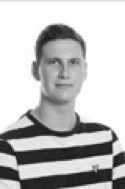
\includegraphics[width=0.15\textwidth]{adamjacobs}
       \end{center}
        \vspace{-1cm}
    \end{wrapfigure}
    
    \section{\mysidestyle Information}%\vspace{2mm}
    Adam Jacobs \\
    tel: +46704799492 \\
    email: $adamjac@kth.se$
    \href{} \\

\section{\mysidestyle Profile}\vspace{1mm}
    I study Computer Science because my goal is to innovate how regular people live and enter a field that requires constant learning throughout life. Leading digital change is my passion! One of my first professional projects was an app for my high school that helped students and teachers share their IT knowledge with newly arrived students, which taught me early on that nothing changes by itself - take initiatives and learn what you need to change the world!  
In my free time I enjoy staying updated with current events, playing drums and singing with my band in order to relieve stress for the next week. I also continuously reflect upon what I've learnt and done the latest time, in order to get new ideas and always be one step ahead.

\section{\mysidestyle Core Values}\vspace{1mm}
    My favourite thing is developing awesome things by constantly learning, which is reached by following my core values: 
    \\
    \\
    \textbf{Diversity} helps us empower each other with many different experiences which is needed in our complicated world
    \\
    \textbf{Rethink} what you are doing. Being able to stop and reflect and perhaps change your ways is an important aspect.
    \\
    \textbf{Performance} is achieved via effort and not how smart you are. There are no limits.

\section{\mysidestyle Education}\vspace{1mm}
    \begin{description}
        \item[KTH Computer Science] (2016-2021)
        \item[Technology] Rudbeck Gymnasium in Sollentuna (2013-2016)
        \item[Leadership] course for children summer camps (2014-2015)
    \end{description} 

\section{\mysidestyle Projects and Volountering}\vspace{1mm}
\begin{description}
    \item[Personal Projects] https://github.com/worldyn
    \item[Soft. Eng] course, team leader for 11 people, company Greenlytics.   
     \item[System Developer] THS Armada Career Fair
    \item[App Developer] Rudbeck (Awarded for best school tech project) 

\end{description}  
  
\section{\mysidestyle Work Exp.}\vspace{1mm}
\begin{description}
    \item[Network Software] Engineer, Ericsson Internship, product in prototype-stage
    \item[Freelancing/Consultant] Built and sold task management system to schools
    \item[Ceremony] host at Fonus. Handling grieving people.
    \item[Freelancing] multi-platform app, digitalizing education, Rudbeck 
    \item[Freelancing] Web developer for UF-companies
    \item[Sales] Clas Ohlson Internship
\end{description}

\section{\mysidestyle References}
\begin{description}
    \item[Linkedin] https://www.linkedin.com/in/adam-jacobs-7a7820139/
    \item[Written] references handed in per request.
\end{description}

\end{resume}
\end{document} 